\documentclass[a4paper, 11pt]{article}

\usepackage[czech]{babel}
\usepackage[utf8]{inputenc}
\usepackage[left=2cm, top=3cm, text={17cm, 24cm}]{geometry}
\usepackage{times}
\usepackage{multirow}
\usepackage[ruled, czech, linesnumbered, noline, longend]{algorithm2e}
\usepackage{graphics}
\usepackage{pdflscape}
\usepackage{hyperref}
\hypersetup{
    colorlinks=true,
    linkcolor=blue,
    filecolor=magenta,      
    urlcolor=cyan,
    pdftitle={Overleaf Example},
    pdfpagemode=FullScreen,
    }

\begin{document}

	\begin{titlepage}
		\begin{center}
			\LARGE\textsc{Vysoké učení technické v~Brně} \\
			\Large\textsc{Fakulta informačních technologií}\\
			\vspace{\stretch{0.382}}
			\Large{Seminář VHDL -- dokumentace k finálnímu projektu}
			\vspace{\stretch{0.618}}
		\end{center}

		\Large{18. května 2021 \hfill Vojtěch Kališ (xkalis03)}
	\end{titlepage}

	%pic
	\begin{figure}[h]
		\centering
		\scalebox{0.8}{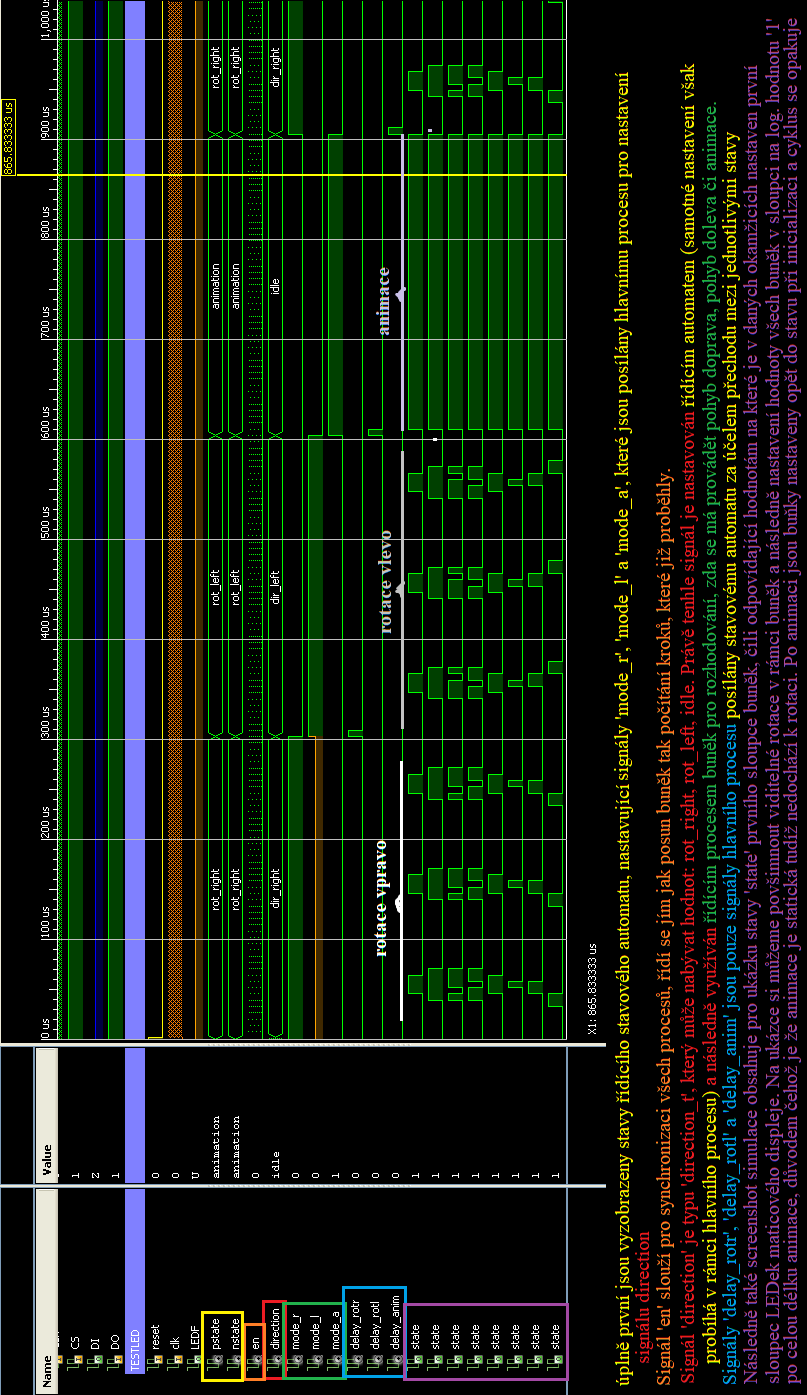
\includegraphics{ivh_sim.png}}
		\caption{Screenshot výstupu simulace}
		\label{obr}
	\end{figure}

	\vspace*{\stretch{0.4}}

	\hspace*{4.5cm}\textbf{\Large \centering Zdůvodnění použitých konstant} \\		
	\begin{itemize}
		\item \emph{constant CLK\_FREQ = 25000000 (lumin\_board.vhd)}: vstupní frekvence CLK 25MHz
		\item \emph{constant OUT\_FREQ = 15 (lumin\_board.vhd)}: výstupní frekvence (15 přechodů za sekundu)
		\item \emph{signal mov\_cnt : integer range 0 to 143 (lumin\_board.vhd)}: čítač používán při rozhodování momentálního stavu displeje, je prováděno 3*16 kroků doprava, 3*16 kroků doleva, a animace trvá 3*16 \uv{kroků} taktéž, čili 3*48 = 144-1 = 143
		\item \emph{signal cnter = integer range 0 to 47 (cell.vhd)}: využíván k počítání do posledního kroku při animaci, v tento moment se totiž musí signál 'state' u všech buněk nastavit opět na původní hodnotu jinak by rotace byla prováděna s výstupem animace (rotovalo by se s výstupem animace)
		\item \emph{constant delay1 = 3999 (display.vhd)}: určuje počet CLK+1, po jejichž, dobu se bude držet rozsvěcený jeden sloupec displeje než se přejde na rozsvěcení sloupce vedlejšího. K nalezení konstanty došlo zkoušením konstant, dokud displej nepřestal blikat
	\end{itemize}

	\vspace*{\stretch{0.2}}

	\hspace*{4cm}\textbf{\Large \centering Odkaz na video s komentářem je \href{https://drive.google.com/file/d/150QRpHBC9p5e2X4qCt9Scvb0kyMNy3he/view?usp=sharing}{zde}} \\ \\
	\noindent Omlouvám se, jsem si vědom faktu že video je poněkud \uv{zasekané} (zvukový výstup je naštěstí v pořádku), avšak nepodařilo se mi natočit video lepší kvality, jelikož jediný počítač který mám momentálně k dispozici není úplně nejrychlejší a točit skrze mobilní telefon by dle mého nedopadlo o moc lépe.

	\vspace*{\stretch{0.4}}

	

	\newpage


\end{document}


